\documentclass[12pt]{amsart}

\usepackage{tikz}
\usepackage{bbm}
\usetikzlibrary{3d,arrows,calc,positioning,decorations.pathreplacing,matrix} %,arrows.meta}

\usepackage{calligra,mathrsfs}
\usepackage[all]{xy}
\usepackage{float, comment}
\usepackage{mathtools}
\usepackage{amsmath}
\usepackage{amsthm}
\usepackage{amssymb}
\usepackage{amsbsy}
\usepackage{amstext}
\usepackage{amsopn}
%\usepackage{mathrsfs} % allows \mathscr
\usepackage[mathscr]{eucal}
\usepackage{enumerate}
\usepackage{xcolor}
\usepackage{graphicx} % allows \includegraphics{}s
\usepackage{scalerel}
\usepackage{microtype} % improves formattings
\usepackage[margin=1in,marginparwidth=0.8in, marginparsep=0.1in]{geometry}
\renewcommand{\baselinestretch}{1.2} % changes page formatting
\usepackage[pagebackref, bookmarks=true, bookmarksopen=true, bookmarksdepth=3,bookmarksopenlevel=2, colorlinks=true, linkcolor=blue, citecolor=blue, filecolor=blue, menucolor=blue, urlcolor=blue]{hyperref}
% \usepackage{newtxtext} % improves font appearance
\usepackage{tikz}
\usepackage{bbm}
\usepackage[all]{xy}
\usetikzlibrary{arrows,calc,positioning,decorations.pathreplacing} %,arrows.meta}

\usepackage{tikz-cd}
\hypersetup{
    colorlinks=true,
    citecolor=red,
    linkcolor=blue,
    urlcolor=red,
}
\usepackage[capitalize, nameinlink]{cleveref}

\numberwithin{equation}{section}
\newtheorem{Theorem}[equation]{Theorem}
\newtheorem{Proposition}[equation]{Proposition} 
\newtheorem{Lemma}[equation]{Lemma}
\newtheorem{Open}[equation]{Open Question}
\newtheorem{Corollary}[equation]{Corollary}
\newtheorem{Conjecture}[equation]{Conjecture}
\newtheorem{Specialthm}{Theorem}
\newtheorem{Question}{Question}

\theoremstyle{definition}
\newtheorem{Remark}[equation]{Remark}
\newtheorem{Example}[equation]{Example}
\newtheorem{Definition}[equation]{Definition}

\numberwithin{figure}{section}

\def\la{\langle}
\def\ra{\rangle}
\def\ttimes{\widetilde{\times}}
\def\tbox{\widetilde{\boxtimes}}
\def\bbox{{\boxtimes}}
\def\O{\mathcal{O}}
\def\K{\mathcal{K}}
\def\bG{\mathbb{G}}
\newcommand{\gr}{\mathrm{gr}}
\newcommand{\mb}[1]{\mathbf{#1}}
\newcommand{\fsl}{\mathfrak{sl}}
\newcommand{\fg}{\mathfrak{g}}
\newcommand{\fn}{\mathfrak{n}}
\newcommand{\bk}{{\mathbbm k}}
\newcommand{\A}{\mathbb{A}}
\newcommand{\C}{\mathbb{C}}
\newcommand{\D}{\mathbb{D}}
\newcommand{\E}{\mathbb{E}}
\newcommand{\G}{\mathbb{G}}
\newcommand{\bN}{\mathbb{N}}
\renewcommand{\P}{\mathbb{P}}
\newcommand{\Q}{\mathbb{Q}}
\newcommand{\Z}{\mathbb{Z}}
\newcommand{\bfC}{{\mathbf{C}}}
\newcommand{\bfD}{{\mathbf{D}}}
\newcommand{\bfI}{{\mathbf{I}}}
\newcommand{\cA}{\mathcal{A}}
\newcommand{\cB}{\mathcal{B}}
\newcommand{\cC}{\mathcal{C}}
\newcommand{\cD}{\mathcal{D}}
\newcommand{\cE}{\mathcal{E}}
\newcommand{\cF}{\mathcal{F}}
\newcommand{\cG}{\mathcal{G}}
\newcommand{\cH}{\mathcal{H}}
\newcommand{\cK}{\mathcal{K}}
\newcommand{\cL}{\mathcal{L}}
\newcommand{\cM}{\mathcal{M}}
\newcommand{\cN}{\mathcal{N}}
\newcommand{\cO}{\mathcal{O}}
\newcommand{\cP}{\mathcal{P}}
\newcommand{\cQ}{\mathcal{Q}}
\newcommand{\cR}{\mathcal{R}}
\newcommand{\cS}{\mathcal{S}}
\newcommand{\cT}{\mathcal{T}}
\newcommand{\cU}{\mathcal{U}}
\newcommand{\cV}{\mathcal{V}}
\newcommand{\cW}{\mathcal{W}}
\newcommand{\cX}{\mathcal{X}}
\newcommand{\cY}{\mathcal{Y}}
\newcommand{\sW}{\mathscr{W}}
\newcommand{\sX}{\mathscr{X}}
\newcommand{\sY}{\mathscr{Y}}
\newcommand{\sZ}{\mathscr{Z}}

\newcommand{\hs}{\heartsuit}
\newcommand{\bul}{\bullet}
\newcommand{\ga}{\gamma}
\newcommand{\al}{\alpha}
\newcommand{\be}{\beta}

%% code from mathabx.sty and mathabx.dcl
\DeclareFontFamily{U}{mathx}{\hyphenchar\font45}
\DeclareFontShape{U}{mathx}{m}{n}{
	<5> <6> <7> <8> <9> <10>
	<10.95> <12> <14.4> <17.28> <20.74> <24.88>
	mathx10
}{}
\DeclareSymbolFont{mathx}{U}{mathx}{m}{n}
\DeclareFontSubstitution{U}{mathx}{m}{n}
\DeclareMathAccent{\widecheck}{0}{mathx}{"71}
\DeclareMathSymbol{\shortminus}{\mathbin}{AMSa}{"39}

\DeclareRobustCommand{\SkipTocEntry}[5]{}

\newcommand{\arrtip}{latex'}

%Custom commands

\newcommand{\grass}[2]{\mathrm{Gr}(#1,#2)}
\newcommand{\fl}{\mathcal{FL}}
\newcommand{\gl}{\mathrm{GL}}
\newcommand{\attr}{\mathrm{attr}}
\newcommand{\attrl}{\mathrm{attrlang}}
\newcommand{\set}[1]{\left\{ #1 \right\}}
\newcommand{\paren}[1]{\left( #1 \right)}

\newenvironment{ccd}{\begin{center}
\begin{tikzcd}}{\end{tikzcd}
\end{center}}

\tikzset{gauged/.style={rectangle,rounded corners=2mm,draw,inner sep=1mm,minimum size=4mm}}
\tikzset{framed/.style={rectangle,draw,inner sep=0.5mm,minimum size=4mm}}
\tikzset{script math mode/.style = {execute at begin node=$ , execute at end node=$}}
\newcommand\dOne[2]{
\node[gauged] at (1,0) (v1) {#1}; 
\node[gauged] at (2,0) (v2) {#2}; 
\draw (v1) -- (v2);
}

\begin{document}
\title{Notes on Schubert Calculus and Quantum Integrability}

\begin{abstract}
\end{abstract}

\maketitle

\setcounter{tocdepth}{1}

\tableofcontents

\section{Introduction}

\thispagestyle{empty}

Here is a template for a simple commutative diagram in tikz:
\begin{equation*}
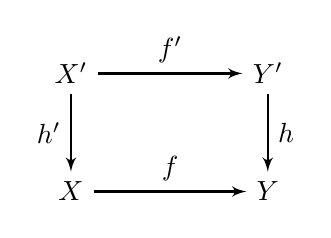
\begin{tikzpicture}
[baseline=(current  bounding  box.center),thick,>=\arrtip]
\node (a) at (0,0) {$X'$};
\node (b) at (2.5,0) {$Y'$};
\node (c) at (0,-1.5) {$X$};
\node (d) at (2.5,-1.5) {$Y$};
\draw[->] (a) to node[above] {$f' $} (b);
\draw[->] (b) to node[right] {$h $} (d);
\draw[->] (a) to node[left] {$h' $}(c);
\draw[->] (c) to node[above] {$f $} (d);
\end{tikzpicture}
\end{equation*}

Here is a template for an elaborate commutative diagram in tikz:
\begin{equation*}
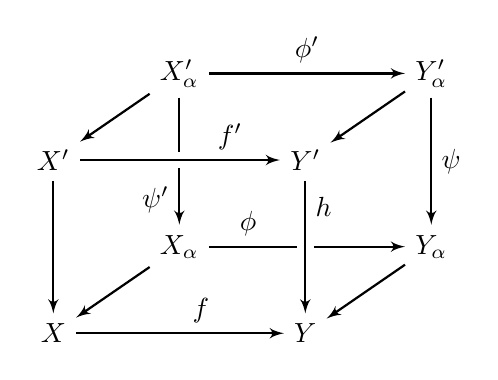
\begin{tikzpicture}[baseline=(current  bounding  box.center),thick,>=\arrtip]
\newcommand*{\ha}{1.6}; \newcommand*{\hb}{1.6}; \newcommand*{\hc}{1.6};
\newcommand*{\va}{-1.1}; \newcommand*{\vb}{-1.1}; \newcommand*{\vc}{-1.1};
\node (ab) at (\ha,0) {$X_\al'$};
\node (ad) at (\ha+\hb+\hc,0) {$Y_\al'$};
\node (ba) at (0,\va) {$X'$};
\node (bc) at (\ha+\hb,\va) {$Y'$};
\node (cb) at (\ha,\va+\vb) {$X_\al$};
\node (cd) at (\ha+\hb+\hc,\va+\vb) {$Y_\al$};
\node (da) at (0,\va+\vb+\vc) {$X$};
\node (dc) at (\ha+\hb,\va+\vb+\vc) {$Y$};
\draw[->] (ab) to node[above] {$\phi' $} (ad);
\draw[->] (ab) to node[above] {$ $} (ba);
\draw[->] (ab) to node[left,pos=.8] {$\psi' $} (cb);
\draw[->] (ad) to node[above] {$ $} (bc);
\draw[->] (ad) to node[right] {$\psi $} (cd);
\draw[->] (ba) to node[above] {$ $} (da);
\draw[->] (cb) to node[above,pos=.2] {$\phi $} (cd);
\draw[->] (cb) to node[above] {$ $} (da);
\draw[->] (cd) to node[above] {$ $} (dc);
\draw[->] (da) to node[above,pos=.6] {$f $} (dc);

\draw[-,line width=6pt,draw=white] (ba) to  (bc);
\draw[->] (ba) to node[above,pos=.75] {$f' $} (bc);
\draw[-,line width=6pt,draw=white] (bc) to  (dc);
\draw[->] (bc) to node[right,pos=.2] {$h $} (dc);
\end{tikzpicture}
\end{equation*}

\section{Lecture 1 (Allen Knutson)}

\section{Lecture 2 (Allen Knutson)}

\section{Lecture 3 (Paul Zinn-Justin)}

\section{Lecture 4 (Paul Zinn-Justin)}

\section{Lecture 5 (Allen Knutson)}

\section{Lecture 6 (Allen Knutson)}

\section{Lecture 7 (Paul Zinn-Justin)}

\section{Lecture 8 (Paul Zinn-Justin)}

\section{Lecture 9 (Allen Knutson)}

\section{Lecture 10 (Allen Knutson)}

\section{Lecture 11 (Paul Zinn-Justin)}

\section{Lecture 12 (Paul Zinn-Justin)}

\section{Lecture 13 (Allen Knutson)}

\section{Lecture 14 (Paul Zinn-Justin)}

\section{Lecture 15 (Allen Knutson)}

\section{Lecture 16 (Allen Knutson)}

\subsection{Setup}
\hfill\\
Consider the diagonal embedding $\grass{k}{n}\xrightarrow{\Delta}\grass{k}{n}\times \grass{k}{n}$. Recall from Knutson 7 that any continuous map between varieties/manifolds gives the following commutative diagram in the category of correspondences
\begin{ccd}
 \grass{k}{n}\times \grass{k}{n} \ar[d, "graph(s)\times graph(s) ", swap]   \ar[r, "graph(\Delta)^T"] & \grass{k}{n}  \ar[d, "graph(s)"] \\
 T^*\grass{k}{n}\times T^* \grass{k}{n}\ar[r, "C_{graph(\Delta)^T}"] & T^*\grass{k}{n}
\end{ccd}
where composition is given by fiber product, $s: \grass{k}{n}\hookrightarrow T^*\grass{k}{n}$ is the inclusion of the zero section and given $A$ a correspondence in $M\times N$, $C_A$ is the conormal bundle of $A$ in $M\times N$. As it will turn out, we have a better understanding of $C_{graph(\Delta)^T}$ over $graph(\Delta)^T$. \\

Recall that given a correspondence $L\subset M\times N$ we have an induced map on (equivariant) cohomology\footnote{This should really be (equivariant) Borel-Moore homology but for smooth varieties Borel-Moore homology is isomorphic to cohomology via Poincare duality and $\grass{k}{n}$ is smooth.} $\beta_L: H^*(M)\to H^*(N)$ given by the pull-push construction, i.e.
\[  \beta_L(\alpha)=(\pi_N)_* ([L]\cup \pi^*_M([\alpha])) \]
Moreover one has that $\beta_{graph(f)}=H^*(f)$ and in particular we see that $\beta_{graph(s)}:H^*(\grass{k}{n})\to H^*(T^*\grass{k}{n})$ corresponds to multiplication by the Poincare dual of the zero section, so multiplication by 1 for ordinary cohomology. Also recall that the product in (equivariant) cohomology comes from the pullback map of $\Delta$. As such, the transpose/dual map in (equivariant) Borel-Moore homology is given by $\beta_{graph(\Delta)^T}$. Therefore commutativity of the above diagram tells us that the product in $H^*(\grass{k}{n})$ can be computed from the map
\[ \beta_{C_{graph(\Delta)^T}}:H^*( T^*\grass{k}{n})\otimes H^*(T^* \grass{k}{n} )\to H^*( T^*\grass{k}{n})  \]
Switching to $T\times \C^\times$ equivariant cohomology, the only thing that changes is that the class of the Poincare dual of the zero section is no longer trivial so that $\beta_{graph(s)}$ is no longer trivial. Thus if we know the structure constants for multiplication of the Maulik Okounkov classes in $H^*_{T\times \C^\times}( T^*\grass{k}{n})$, say
\[  [MO_\lambda]\cdot [MO_{\mu}]=\sum_\nu \widetilde{c^\nu_{\lambda \mu}} [MO_\nu] \]
it follows from commutativty of the diagram above that in $H^*_{T\times \C^\times}( \grass{k}{n})$ we have the formula
\[  \frac{[MO_\lambda]}{[s]}\cdot \frac{[MO_{\mu}]}{[s]}=\sum_\nu \widetilde{c^\nu_{\lambda \mu}} \frac{[MO_\nu]}{[s]} \]

\begin{Definition}
The Serge-Schwartz-MacPherson class associated to a sequence $\lambda$ is
\[ SSM_\lambda:= \frac{[MO_\lambda]}{[s]}  \]
\end{Definition}

One might think that the classes $SSM_\lambda$ correspond to Schubert classes, but notice that both $[MO_\lambda]$ and $[s]$ arise geometrically from classes of Langrangian subvarieties of $T^*\grass{k}{n}$ and so $SSM_\lambda$ has degree 0. However it will turn out that

\begin{Proposition}
Let $\mathrm{inv}(\lambda)$ be the number of inversions in the sequence $\lambda$. Then
\[  \underset{h\to 0}{\mathrm{lim}} \ h^{\mathrm{inv}(\lambda)} SSM_\lambda=S_\lambda \]
where $S_\lambda$ is the corresponding Schubert class associated to $\lambda$. 
\end{Proposition} 


Heruistically, this is saying that the Schubert classes are the 5 vertex limit of the Maulik Okounkov classes which correspond to the 6 vertex model. 

\subsection{Stable Envelope}
\label{stablesect}
\hfill\\
The reason why we have a better understanding of $C_{graph(\Delta)^T}$ is that it factors 
\begin{ccd}
T^*\grass{k}{n}\times T^*\grass{k}{n} \ar[rd,"senv", swap] \ar[rr, "C_{graph(\Delta)^T}"]& & T^*\grass{k}{n} \\
& T^* \fl(k, n+k; 2n) \ar[ur,"hr", swap] &
\end{ccd}
Let us first describe the first correspondence/map $senv$, the stable envelope. 

\begin{Definition}
Let $\C^\times$ act on a variety $M$. Then define
\[ \attr(M, \C^\times)=\set{ m\in M \left\vert \, \lim_{z\to 0} z \cdot m \textnormal{  exists} \right.} \]
and similarly define 
\[\attrl(M, \C^\times)=\set{ (m_\ell, m)\in M^{\C^\times}\times M \left\vert \, m_\ell=\lim_{z\to 0} z \cdot m \textnormal{  exists} \right.} \]
\end{Definition}


\begin{Remark}
If $M$ is compact, then $\attr(M)=M$. When $M$ is not compact then $\attr(M)$ can be quite small. For example, let $\C^\times$ act on $\C$ with weight $-1$. Then only the origin $(0,0)$ is in $\attr(M)$, the limit for everything else goes to infinity.  
\end{Remark}

\begin{Remark}
$\attrl(M, \C^\times)$ is a correspondence between $M^{\C^\times}$ and $M$, but isn't the one we are looking for because the map $\attrl(M, \C^\times)\to M$ need not be proper\footnote{And so there will be no pushforward map in Borel-Moore homology}! For example, let $\C^\times$ act on $\C\P^1$ by $z\cdot [a: b]=[za:b]$. $\C\P^1$ is compact, so $\attr(M)=M$. Moreover, one can check that the only fixed points are $[1:0]$ (north pole) and $[0:1]$ (south pole) and that $m_\ell=[0:1]$ for all points $m\in \C\P^1$ except the north pole. It follows that $\attrl(M, \C^\times)=\C\sqcup pt$ topologically, and this isn't compact and so the map $\attrl(M, \C^\times)\to M$ cannot be proper in this case.
\end{Remark}

\begin{Theorem}
\label{affinetheorem}
If $M$ is affine, then the map $\attrl(M, \C^\times)\to M$ is proper.
\end{Theorem}

The following example will be very important. 

\begin{Example}
Let 
$$M^\prime=\mathrm{GL}_n\cdot\begin{pmatrix}
\epsilon_1 I_{n_1} &  &  &  \\
& \epsilon_2 I_{n_2} & & \\
 &  & \ddots &  \\
 &  &  & \epsilon_d I_{n_d}
\end{pmatrix}$$ where $\mathrm{GL}_n$ acts by conjugation and all the $\epsilon_i$ are fixed distinct elements of $\C$. This is what the general fiber of the partial Grothendieck Springer resolution $\mathrm{GS}_{n_1, \ldots, n_d}$ looks like. Recall that
\[ M^\prime\cong \frac{\gl_n}{\gl_{n_1}\times \ldots \gl_{n_d}} \]
And as a result, $M$ will be an affine variety as it's the quotient of a reductive group acting on an affine variety. 
\end{Example}

Now, consider the case when $M=T^*\fl(k, n+k; 2n)$. This is not affine and so we can't use \cref{affinetheorem} to conclude that $\attrl(M, \C^\times)$ gives rise to a map in cohomology. However, recall that $M$ is the 0 fiber in the partial Grothendieck Springer resolution, i.e.
\[  \mathrm{GS}_{k, n+k}|_{\vec{\epsilon}=\vec{0}} = T^*\fl(k, n+k; 2n) \]

So $M$ in this case is the limit or special fiber of a family of varieties, most of which are affine by the example above (the set of points whose fibers are affine are dense). Therefore if we define 
\begin{Definition}
\[ env:=\lim_{\vec{\epsilon}\to \vec{0}} \  \attrl(T^*\fl(k, n+k; 2n), \C^\times ) \]
\end{Definition}
this will give rise to a map
\[ H^*(T^*\fl(k, n+k; 2n)^{\C^\times})\xrightarrow{\beta_{env}} H^*(T^*\fl(k, n+k; 2n)) \]

But what is $T^*\fl(k, n+k; 2n)^{\C^\times}$? Well, this will depend on the weights of the action of $\C^\times$ on $\C^{2n}$, but first consider an easier, related problem, namely $\grass{k}{V\oplus W}$ where $\C^\times$ acts on $V\oplus W$ with weights $0$ on $V$ and $1$ on $W$. Explicitly this means that $z\cdot(\vec{v}, \vec{w})=(\vec{v}, z\vec{w})$. Then because $\C^\times$ acts on $V$ and $W$ with different weights, we will have the following decomposition
\begin{equation}
\label{eq1}
\grass{k}{V\oplus W}^{\C^\times}=\bigsqcup_{i+j=k} \grass{i}{V}\times \grass{j}{W} 
\end{equation}  
One way to get an element of the LHS is the following procedure. Consider any subspace $A\subseteq V\oplus W$ and note that
\[ \lim_{z\to 0} z\cdot A=(\textnormal{Projection of }A \textnormal{ to }V)\oplus A\cap W``=" \mathrm{gr}(A) \]
The notation $\mathrm{gr}(A) $ is because we can think of the result as the associated graded subspace of $A$ under the filtration $0\subseteq W\subseteq V\oplus W$. By \cref{eq1} we see that the LHS above is in $\grass{k}{n}^{\C^\times}$. \\

Now let $V=\C^n$ and $W= \C^n$ and again let $\C^\times$ act on $V$ and $W$ with weights 0 and 1. The same reasoning giving rise to the decomposition in \cref{eq1} also applies to the two step partial flag variety, i.e. we will have the following decomposition
\[ \fl(k, n+k; 2n)^{\C^\times}= \bigsqcup_{\substack{a+c=k \\ b+d=n+k}} \fl(a,b ; n)\times \fl(c,d; n) \]
And notice that for $a=0, b=k$, we have that the RHS above will be
\[ \fl(0,k ; n)\times \fl(k, n ; n)=\grass{k}{n}\times \grass{k}{n} \]
$\grass{k}{n}\times \grass{k}{n}$ is one of the 
Now applying $T^*$ to everything, and since $T^*(\grass{k}{n}\times \grass{k}{n})\hookrightarrow T^* \fl(k, n+k; 2n)^{\C^\times}$ is closed it's also proper and so we obtain our desired map
\[ senv: H^*(T^*( \grass{k}{n})\times T^*(\grass{k}{n}) \, )\to H^*(T^*\fl(k, n+k; 2n)^{\C^\times})\xrightarrow{\beta_{env}} H^*(T^*\fl(k, n+k; 2n)) \] 

\subsection{Hamiltonian Reduction and Nakajima quiver varieties}

\begin{Definition}
Suppose that $G$ is a Lie group acting on symplectic manifold $M$ such that the action is Hamiltonian. Let $\mu: M\to \mathfrak{g}^*$ be the associated moment map and let $\lambda$ be a regular value of $\mu$. Then the symplectic reduction is defined to be $\mu^{-1}(\lambda)/G$. If $\lambda$ and $\mu$ are given, this will be abbreviated as $M//G$.
\end{Definition}

\begin{Theorem}[Marsden-Weinstein]
$M//G$ is a symplectic manifold. 
\end{Theorem}

\begin{Theorem}
If $G$ is compact, the quotient map $\pi: \mu^{-1}(\lambda)\to M//G$ is proper.
\end{Theorem}
\begin{proof}
We need to show that $\pi$ is closed with compact fibers. The fact that $\pi$ is closed reduces to the fact that when $G$ is compact, the $G-$orbit of a closed set is also a closed set. The fibers of $\pi$ are all of the form $G\cdot m$ where $m\in M$ which is diffeomorphic to $G/ G_m$ where $G_m$ is the stabilizer of $m$. Since $G$ is compact, and $G\to G / G_m$ is surjective and continuous, it follows that $G / G_m$ is also compact.  
\end{proof}

Thus when $G$ is compact, it follows from above that $\mu^{-1}(\lambda)\times M//G$ gives us a correspondence from $M$ to the symplectic reduction $M//G$ such that we get an induced map on Borel-Moore homology. Moreover, since $\lambda$ is a regular value, $\mu$ is a submersion at $\lambda$ and it follows that $\mu^{-1}(\lambda)$ has codimension $\dim \mathfrak{g}^*=\dim G$ in $M$. It follows that 
\begin{equation}
\label{dimeq}
\dim M//G=\dim \mu^{-1}(\lambda)-\dim G=\dim M-2\dim G
\end{equation}

We want to apply the formalism above to $M=T^*\fl(k, n+k; 2n)$ so we want to find a compact $G$ such that $M//G=T^*\grass{k}{n}$. First note that 
\[  \fl(k, n+k; 2n)\cong \frac{\gl_{2n}}{  P_{k,n,n-k}  }\qquad \qquad  \grass{k}{n}\cong \frac{\gl_n}{P_{k, n-k} } \]
where $P_{k,n,n-k}$ and $P_{k, n-k}$ are the parabolic subgroups corresponding to the partition $k+n+n-k$ of $2n$ and $k+n-k=n$ of $2n$ and $n$ respectively. As a result, one can then compute their dimensions by computing the dimensions of the tangent spaces resulting in
\[ \dim T^*\fl(k, n+k; 2n) = 2n^2+2k(n-k) \qquad \qquad \dim T^*\grass{k}{n}=2k(n-k) \]

By \cref{dimeq}, it follows that we should have $\dim G=n^2$. So where are we going to find a compact group of dimension $n^2$ acting on $T^*\fl(k, n+k; 2n)$? It turns out that both $T^*\fl(k, n+k; 2n)$ and $T^*\grass{k}{n}$ are Nakajima quiver varieties, and these come with natural actions of $``\gl(\vec{w})"$ on the ``framed" vertices. We won't define these varieties, but will say how these varieties are indexed. Given a Dynkin diagram $I$, construct the Nakajima diagram of $I$ by attaching a framed vertex hanging off each vertex of $I$. For example the Nakajima diagram for $A_4$ looks like 
$$
\tikz[script math mode,baseline=0]{
\node[framed] at (0,1) (w1) { }; 
\node[framed] at (1,1) (w2) { }; 
\node[framed] at (2,1) (w3) { }; 
\node[framed] at (3,1) (w4) { }; 
\node[gauged] at (0,0) (v1) { }; 
\node[gauged] at (1,0) (v2) { }; 
\node[gauged] at (2,0) (v3) { }; 
\node[gauged] at (3,0) (v4) { }; 
\draw (w1) -- (v1) -- (v2) -- (v3) -- (v4) -- (w4);
\draw (w2) -- (v2);
\draw (w3) -- (v3);
}
$$
Given a Nakajima diagram, by filling in the vertices and framed vertices of $I$ with natural numbers with natural numbers $\vec{w}=(w^i)_{i\in I}$ and $\vec{v}=(v^i)_{i\in I}$ , there is a procedure to turn this datum into an algebraic variety $\mathcal{M}(I, \vec{w}, \vec{v})$.  For example,
$$\mathcal{M}(A_1, (n), (k))=
\tikz[script math mode,baseline=0]{
\node[framed] at (0,1) (w1) {n }; 
 \node[gauged] at (0,0) (v1) {k }; 
\draw (w1) -- (v1);
}\ \raisebox{1.4ex}{$\cong T^*\grass{k}{n}$}
$$
We should note that if $w^i=0$ then we will not draw the framed vertex at $i$. In general if $n_1<\ldots<n_{d-1}<n_d$ then we will have that  
$$
\tikz[script math mode,baseline=0]{
\node[framed] at (0,1) (w1) { n}; 
\node[gauged] at (0,0) (v1) {n_d }; 
\node[gauged] at (1,0) (v2) { n_{d-1}}; 
\node[gauged] at (2,0) (v3) {\ldots }; 
\node[gauged] at (3,0) (v4) { n_1}; 
\draw (w1) -- (v1) -- (v2) -- (v3) -- (v4);
}\ \raisebox{1.4ex}{$\cong  T^*\fl(n_1, \ldots, n_d; n)$}
$$
In our case we will be working with the Nakajima quiver variety 
$$
\tikz[script math mode,baseline=0]{
\node[framed] at (0,1) (w1) { 2n}; 
\node[gauged] at (0,0) (v1) {n+k}; 
\node[gauged] at (1.3,0) (v2) { k}; 
\draw (w1) -- (v1) -- (v2);
}\ \raisebox{1.4ex}{$\cong  T^*\fl(k,  n+k; 2n)$}
$$
The framed vertex $\tikz[script math mode, baseline=(w1.base)]{
\node[framed] at (0,0) (w1) { 2n}; 
}$ has an action of $\gl_{2n}$. If we write $T^*\fl(k,  n+k; 2n)$ in Springer coordinates, e.g.
\[ T^*\fl(k,  n+k; 2n)=\set{(X, V^{n+k}\supset W^k)\, | \, X\in \mathrm{End}(\C^{2n}), \C^{2n}\xrightarrow{X} V^{n+k}\xrightarrow{X}W^k\xrightarrow{X} 0 } \]
where $V^{n+k}$ is a $n+k$ dimensional subspace of $\C^{2n}$ and $W^k$ is a $k$ dimensional subspace in $V^{n+k}$, then the action of $g\in \gl_{2n}$ is
\begin{equation}
\label{actioneq}
g\cdot( X, V^{n+k}\supset W^k)=(gxg^{-1}, g( V^{n+k})\supset g(W^k)) 
\end{equation}  
Inside $\gl_{2n}$ we have the unitary subgroup 
\[ U_n:=\left\{ \left.\begin{bmatrix}
I_n & 0 \\
E & I_n
\end{bmatrix} \right\vert  E\in \mathrm{Mat}_{n\times n}  \right\} \subseteq \gl_{2n}\]
which is a compact group of dimension $n^2$ so this fits our criteria from above. The moment map for the action of $U_n$ turns out to send $X$ to the northeast $n\times n$ quadrant of $X$ when written in block matrix form. We will let $\lambda=I_n$ and as a result we have that
\[  T^*\fl(k,  n+k; 2n)//U_n= \set{(X, V^{n+k}\supset W^k)\, \left \vert  X=\begin{bmatrix}
A & I_n \\
C & D
\end{bmatrix},  \C^{2n}\xrightarrow{X} V^{n+k}\xrightarrow{X}W^k\xrightarrow{X} 0 \right.} /U_n \]

\begin{Proposition}
\[  T^*\fl(k,  n+k; 2n)//U_n\cong T^*\grass{k}{n} \]
\end{Proposition}
\begin{proof}
The fiber of the moment map imposes more conditions on the set of tuples $(X, V, W)$ than described above. In particular, let $\vec{v}=(\vec{v_1} \ \vec{v_2})^T\in \ker X$. Then it follows from
\[ \begin{bmatrix}
A & I_n \\
C & D
\end{bmatrix}\begin{pmatrix}
\vec{v_1}\\
\vec{v_2}
\end{pmatrix}=\begin{pmatrix}
A\vec{v_1}+\vec{v_2}\\
C\vec{v_1}+D\vec{v_2}
\end{pmatrix} =\begin{pmatrix}
0 \\
0
\end{pmatrix}
\]
that $\vec{v_2}=-A\vec{v_1}$ and thus $(C-DA)\vec{v_1}=0$. We claim that $\dim \ker X\ge n$ from which it follows that $(C-DA)\vec{v_1}=0 \ \forall \vec{v_1}\in \C^n$ or in other words $C=DA$. Because $X$ preserves the flag, $X$ restricts to a map
\[  X|_V: V\to W \]
Because $\dim V=n+k$ and $\dim W=k$, by rank-nullity it follows that
\[ \dim \ker X|_V=(n+k)-\dim \mathrm{im } X|_V\ge (n+k)-k=n \]
and thus $C=DA$ as desired. In fact much more is true, as from before we know that
\[  \ker X \subseteq \set{\begin{bmatrix}
v \\
-Av
\end{bmatrix}, v\in \C^n}=V_0\]
and the subspace on the right has dimension $n$. Therefore 
$$\dim \ker X=\dim \ker X|_V=n\implies\ker X =V_0\subseteq V \textnormal{ and } \mathrm{im }X|_V=W $$
Another consequence of the moment map condition is that since $X^3=0$ we have
\[ X^3=\begin{bmatrix}
* & C+A^2+AD+D^2 \\
* & *
\end{bmatrix} = 0\]
As $C=DA$ the top right entry will be $(A+D)^2$ and so $(A+D)^2=0$. \\

We now consider the action of $U_n$. We claim that any element in 
$\mu^{-1}(I_n)$ is in the orbit of elements of the form
\[  \left( X=\begin{bmatrix}
0 & I_n \\
0 & F
\end{bmatrix} , \C^n\oplus M \supset X(M) \right) \]
Given $(X, V^{n+k}\supset W^k)\in \mu^{-1}(I_n)$, let $V^{\prime}:=(0\oplus \C^n)\cap V$. We claim that $ V=\ker X\oplus V^\prime $. The above description of $\ker X=V_0$ shows that $\ker X\cap V^\prime=\set{0}$ and it is easy to see that these two subspaces span $V$. From this we see that $X|_{V^\prime}$ gives an isomorphism $V^\prime\xrightarrow{\simeq}W$ and thus $W$ is extraneous data, as it can be recovered from $X$ and $V$. Let $g=\begin{bmatrix}
I_n & 0 \\
A & I_n
\end{bmatrix}$. By the definition of the action \cref{actioneq} one can compute that
\[ g\cdot(X, V)=g\cdot \paren{ \begin{bmatrix}
A & I_n\\
DA & D
\end{bmatrix} , \ker X\oplus V^\prime }=  \paren{ \begin{bmatrix}
0 & I_n\\
0 & A+D
\end{bmatrix} , \C^n\oplus V^\prime}\]
which is exactly of the form above. Now, the RHS only depends on the datum of $A+D$ and $V^\prime$ and we claim that they in fact satisfy the conditions to be in $T^*\grass{k}{n}$. As $(A+D)^2=0$ from above, we only need to check that $(A+D)v\in V^\prime\ \forall v\in \C^n$. This follows from $V_0\subset V$ and so 
\[ \begin{pmatrix}
0 \\
(A+D)v
\end{pmatrix}=\begin{pmatrix}
v \\
Dv
\end{pmatrix}-\begin{pmatrix}
v \\
-Av
\end{pmatrix}\in V \]
\end{proof}

\subsection{Finale}


As explained in the paragraph before \cref{dimeq}, the Hamiltonian reduction now gives us a correspondence
\[ hr:  T^*\fl(k,  n+k; 2n)\to  T^*\grass{k}{n}   \]
and as alluded to at the beginning of \cref{stablesect} we have the following theorem

\begin{Theorem}[\href{https://arxiv.org/pdf/2102.00563.pdf}{Knutson, Zinn-Justin, 2021}]
  The two Lagrangian correspondences $senv,hr$
  $$
  \tikz[script math mode,baseline=0]{\dOne{k}{0} 
    \node[framed] at (1,1) (w1) {n}; \draw (v1) -- (w1);}
  \quad\times\quad
  \tikz[script math mode,baseline=0]{\dOne{n}{k} 
    \node[framed] at (1,1) (w1) {n}; \draw (v1) -- (w1);}
  \quad \xrightarrow{senv}
  \phantom{   \prod\limits_{i=1}^{n} }
  \tikz[script math mode,baseline=0]{\dOne{n+k}{k} 
    \node[framed] at (1,1) (w1) {2n}; \draw (v1) -- (w1);} 
  \quad  \xrightarrow{hr} % \xrightarrow{///_{I_n} U}
  \quad
  \tikz[script math mode,baseline=0]
  {
    \node[gauged] at (1,0) (v1) {k}; 
    \node[gauged] at (2,0) (v2) {k}; \draw (v1) -- (v2);
    \node[framed] at (2,1) (w2) {n}; \draw (v2) -- (w2);
  }
  $$
  can be composed. Under the identification of first and third spaces
  with $T^* \grass{k}{n}^2$ and $T^* \grass{k}{n}$, 
  the composite is the transpose $C_{graph(\Delta)^T}$ of 
  the conormal bundle of the graph of the diagonal inclusion.
\end{Theorem}

We should note that in order to make the identifications with $T^* \grass{k}{n}$ we are using the following theorem of Nakajima,

\begin{Theorem}[\href{https://link.springer.com/article/10.1007/s00208-003-0467-0}{Nakajima, 2003}] Let $i\in I$,  define 
$$r_i(\vec{v})^j:= \begin{cases}
  \vec{v}^j & \textnormal{ if }j\neq i\\
  \textnormal{sum of all adjacent labels }-\vec{v}^i & \textnormal{ if }j=i
\end{cases}
  $$
Then 
\[  \mathcal{M}(I, \vec{w}, \vec{v})\cong  \mathcal{M}(I, \vec{w}, r_i(\vec{v})) \]
    as complex varieties, equivariantly w.r.t.\ the framing group action
    $\prod_{i\in I} GL(w^i)$ on both sides. \\
\end{Theorem}
Applying Nakajima's theorem above we find that 
\[   \tikz[script math mode,baseline=0]{\dOne{n}{k} 
    \node[framed] at (1,1) (w1) {n}; \draw (v1) -- (w1);}\ \raisebox{1.7ex}{$\cong$} \ \tikz[script math mode,baseline=0]{\dOne{k}{k} 
    \node[framed] at (1,1) (w1) {n}; \draw (v1) -- (w1);}\ \raisebox{1.7ex}{$\cong$} \ \tikz[script math mode,baseline=0]{\dOne{k}{0} 
    \node[framed] at (1,1) (w1) {n}; \draw (v1) -- (w1);} \qquad \qquad   \tikz[script math mode,baseline=0]
  {
    \node[gauged] at (1,0) (v1) {k}; 
    \node[gauged] at (2,0) (v2) {k}; \draw (v1) -- (v2);
    \node[framed] at (2,1) (w2) {n}; \draw (v2) -- (w2);
  } \ \raisebox{1.7ex}{$\cong$} \ \tikz[script math mode,baseline=0]
  {
    \node[gauged] at (1,0) (v1) {0}; 
    \node[gauged] at (2,0) (v2) {k}; \draw (v1) -- (v2);
    \node[framed] at (2,1) (w2) {n}; \draw (v2) -- (w2);
  }\]
\begin{Remark}
We can actually write out the two correspondences very explicitly in Springer coordinates
\begin{gather*}
senv := \left\{ \left(
    (A,V',D,W'),
    \left(X,V,W\right)\right)
  \ :\
  X = \begin{pmatrix} D & * \\ 0 & A \end{pmatrix}, 
  \begin{array}[c]{ccc} V &=& \C^n \oplus V'\\
    W &=& W'\oplus 0  \end{array}
  \right\} 
\\
\begin{matrix}
  \swarrow &&\searrow \\ \\
  \{(A \in \mathrm{End}(\C^n), V'^{\ j})\} \times  \{(D \in \mathrm{End}(\C^n), W'^{\ j})\}
  &\qquad\qquad&
  \left\{ \left(X \in  \mathrm{End}(\C^{2n}), V^{n+j}, W^j \right) \right\}
\end{matrix}
\end{gather*}

$$ 
hr := \left\{ \left((X,V,W),(Y,V'') \right)  \ :\ 
  \begin{array}[c]{c}
    X = \begin{pmatrix} A & Id \\ DA & D \end{pmatrix}, \   Y = A+D\\
    \begin{array}{rcl}
      V \cap (0\oplus \C^n) &=& 0 \oplus V'' \\
      W / (0\oplus \C^n) &=& (W' + \C^n)/(0\oplus \C^n)
    \end{array}
  \end{array}
\right\}   
$$
$$
\begin{matrix}
  \swarrow &&\searrow \\
  \left\{ \left(X \in  \mathrm{End}(\C^{2n}), V^{n+j}, W^j \right) \right\}
  &\qquad\qquad&
  \{(Y \in  \mathrm{End}(\C^n), V''^{\ j})\} 
\end{matrix}
$$

\end{Remark}

\section{Lecture 17 (Paul Zinn-Justin)}

\section{Lecture 18 (Paul Zinn-Justin)}

\end{document}
